\documentclass[12pt]{gatech-thesis}
\usepackage{amsmath,amssymb,latexsym,float,epsfig,subfigure}
%% editing comment

%\newcommand{\cmt}[1]{\textcolor{red}{\textbf {#1}}}
\newcommand{\cmt}[1]{}
\newcommand{\note}[1]{\cmt{Note: #1}}
\newcommand{\karen}[1]{\textcolor{red}{{Karen: #1}}}
\newcommand{\john}[1]{\textcolor{cyan}{{John: #1}}}
\newcommand{\sehoon}[1]{\textcolor{magenta}{{Sehoon: #1}}}
\newcommand{\sehoontext}[1]{\textcolor{magenta}{{#1}}}
\newcommand{\newtext}[1]{#1}
\newcommand{\original}[1]{\textcolor{magenta}{Original: #1}}
\newcommand{\updated}[1]{\textcolor{blue}{Updated: #1}}
\newcommand{\revised}[1]{\textcolor{blue}{#1}}

\newcommand{\myparagraph}[1]{\vspace{0.33cm} \noindent \textbf{#1. }}


%% ignore text
\long\def\ignorethis#1{}

%% abbreviations
\newcommand{\etal}{{\em{et~al.}\ }}
\newcommand{\eg}{e.g.\ }
\newcommand{\ie}{i.e.\ }

%% reference shortcuts
\newcommand{\figtodo}[1]{\framebox[0.8\columnwidth]{\rule{0pt}{1in}#1}}
\newcommand{\figref}[1]{Figure~\ref{fig:#1}}
\newcommand{\tabref}[1]{Table~\ref{tab:#1}}
\newcommand{\eqnref}[1]{Equation~(\ref{eq:#1})}
%\renewcommand{\eqref}[1]{Equation~(\ref{eq:#1})}
\newcommand{\secref}[1]{Section~\ref{sec:#1}}

%% frequently used mathematical structures
\newcommand{\vc}[1]{\ensuremath{\mathbf{#1}}}
\newcommand{\pd}[2]{\ensuremath{\frac{\partial{#1}}{\partial{#2}}}}
\newcommand{\pdd}[3]{\ensuremath{\frac{\partial^2{#1}}{\partial{#2}\,\partial{#3}}}}

%% New commands for Sehoon!
\newcommand{\mat}[1]{\ensuremath{\mathbf{#1}}}
\newcommand{\set}[1]{\ensuremath{\mathcal{#1}}}

% math macros
\newcommand{\vEndEff}{\ensuremath{\vc{d}}}
\newcommand{\vRelMove}{\ensuremath{\vc{r}}}
\newcommand{\sSet}{\ensuremath{S}}


\newcommand{\vControl}{\ensuremath{\vc{u}}}
\newcommand{\vPoint}{\ensuremath{\vc{p}}}
\newcommand{\sSpringCoef}{{\ensuremath{k_{s}}}}
\newcommand{\sDamperCoef}{{\ensuremath{k_{d}}}}
\newcommand{\vHandle}{\ensuremath{\vc{h}}}
\newcommand{\vForce}{\ensuremath{\vc{f}}}

\newcommand{\mTransChain}{\ensuremath{\vc{W}}}
\newcommand{\mRotateTrans}{\ensuremath{\vc{R}}}
\newcommand{\sJoint}{\ensuremath{q}}
\newcommand{\vJoint}{\ensuremath{\vc{q}}}
\newcommand{\mJoint}{\ensuremath{\vc{Q}}}
\newcommand{\mMass}{\ensuremath{\vc{M}}}
\newcommand{\sMass}{\ensuremath{{m}}}
\newcommand{\vGravity}{\ensuremath{\vc{g}}}
\newcommand{\vConstr}{\ensuremath{\vc{C}}}
\newcommand{\sConstr}{\ensuremath{C}}
\newcommand{\vCOM}{\ensuremath{\vc{x}}}
\newcommand{\sGeneralForce}[1]{\ensuremath{Q_{#1}}}
\newcommand{\vStateVar}{\ensuremath{\vc{y}}}
\newcommand{\vControlVar}{\ensuremath{\vc{u}}}
\newcommand{\argmax}{\operatornamewithlimits{argmax}}
\newcommand{\argmin}{\operatornamewithlimits{argmin}}
\newcommand{\tr}[1]{\ensuremath{\mathrm{tr}\left(#1\right)}}




%%%%%%%%%%%%%%%%%%%%%%%%%%%%%%%%%%%%%%%%%%%%%%%%%%%%%%%%%%%%%%%%%%%
%
% Here are a bunch of macros, mostly for math.
%
%%%%%%%%%%%%%%%%%%%%%%%%%%%%%%%%%%%%%%%%%%%%%%%%%%%%%%%%%%%%%%%%%%%

\renewcommand{\choose}[2]{\ensuremath{\left(\begin{array}{c} #1 \\ #2 \end{array} \right )}}

\newcommand{\gauss}[3]{\ensuremath{\mathcal{N}(#1 | #2 ; #3)}}

\newcommand{\pctab}{\hspace{0.2in}}
\newenvironment{pseudocode} {\begin{center} \begin{minipage}{\textwidth}
                             \normalsize \vspace{-2\baselineskip} \begin{tabbing}
                             \pctab \= \pctab \= \pctab \= \pctab \=
                             \pctab \= \pctab \= \pctab \= \pctab \= \\}
                            {\end{tabbing} \vspace{-2\baselineskip}
                             \end{minipage} \end{center}}
\newenvironment{items}      {\begin{list}{$\bullet$}
                              {\setlength{\partopsep}{\parskip}
                                \setlength{\parsep}{\parskip}
                                \setlength{\topsep}{0pt}
                                \setlength{\itemsep}{0pt}
                                \settowidth{\labelwidth}{$\bullet$}
                                \setlength{\labelsep}{1ex}
                                \setlength{\leftmargin}{\labelwidth}
                                \addtolength{\leftmargin}{\labelsep}
                                }
                              }
                            {\end{list}}
\newcommand{\newfun}[3]{\noindent\vspace{0pt}\fbox{\begin{minipage}{3.3truein}\vspace{#1}~ {#3}~\vspace{12pt}\end{minipage}}\vspace{#2}}



\newcommand{\key}{\textbf}
\newcommand{\fun}{\textsc}

\newcommand{\mytilde}{\raise.17ex\hbox{$\scriptstyle\mathtt{\sim}$}}

%\def\shortcite{\def\citename##1{}\@internalcite}

% Local Variables:
% TeX-master: "paper"
% End:


%%
%% This example is adapted from ucthesis.tex, a part of the
%% UCTHESIS class package...
%%
\title{Proposal: \protect\\ Learning dynamic motor skills \protect\\ for virtual and real humanoids} %% If you want to specify a linebreak
                               %% in the thesis title, you MUST use
                               %% \protect\\ instead of \\, as \\ is a
                               %% fragile command that \MakeUpperCase
                               %% will break!
\author{Sehoon Ha}
\department{School of Computer Science}

%% Can have up to six readers, plus principaladvisor and
%% committeechair. All have the form
%%
%%  \reader{Name}[Department][Institution]
%%
%% The second and third arguments are optional, but if you wish to
%% supply the third, you must supply the second. Department defaults
%% to the department defined above and Institution defaults to Georgia
%% Institute of Technology.

\principaladvisor{Professor C. Karen Liu}
%% \committeechair{Professor Ignatius Arrogant}
\firstreader{Professor Greg Turk}
\secondreader{Professor Jarek Rossignac}
\thirdreader{Professor Jun Ueda}[School of Mechanical Engineering]
%% \firstreader{Professor General Reference}[School of Mathematics]
%% \secondreader{Professor Ivory Insular}[Department of Computer Science and Operations Research][North Dakota State University]
%% \thirdreader{Professor Earl Grey}
%% \fourthreader{Professor John Smith}
%% \fifthreader{Professor Jane Doe}[Another Department With a Long Name][Another Institution]
%% %\setcounter{secnumdepth}{2}
\degree{Doctor of Philosophy}

%% Set \listmajortrue below, then uncomment and set this for
%% interdisciplinary PhD programs so that the title page says
%% ``[degree] in [major]'' and puts the department at the bottom of
%% the page, rather than saying ``[degree] in the [department]''

%% \major{Algorithms, Combinatorics, and Optimization} 

\copyrightyear{2014}
\submitdate{April 2014} % Must be the month and year of graduation,
                         % not thesis approval! As of 2010, this means
                         % this text must be May, August, or December
                         % followed by the year.

%% The date the last committee member signs the thesis form. Printed
%% on the approval page.
\approveddate{22 April 2014}

%% \bibfiles{example-thesis}
\bibfiles{proposal}

%% The following are the defaults
%%    \titlepagetrue
%%    \signaturepagetrue
%%    \copyrightfalse
%%    \figurespagetrue
%%    \tablespagetrue
%%    \contentspagetrue
%%    \dedicationheadingfalse
%%    \bibpagetrue
%%    \thesisproposalfalse
%%    \strictmarginstrue
%%    \dissertationfalse
%%    \listmajorfalse
%%    \multivolumefalse

%% Disable the table of contents
\contentspagefalse 
%% Disable the a list of tables
\tablespagefalse
%% Disable the a list of figures
\figurespagefalse

\begin{document}
\bibliographystyle{gatech-thesis}
%%

\begin{preliminary}
%% \begin{dedication}
%% \null\vfil
%% {\large
%% \begin{center}
%% To myself,\\\vspace{12pt}
%% Perry H. Disdainful,\\\vspace{12pt}
%% the only person worthy of my company.
%% \end{center}}
%% \vfil\null
%% \end{dedication}
%% \begin{preface}
%% Theses have elements.  Isn't that nice?
%% \end{preface}
%% \begin{acknowledgements}
%% I want to ``thank'' my committee, without whose ridiculous demands, I
%% would have graduated so, so, very much faster.
%% \end{acknowledgements}
% print table of contents, figures and tables here.
\contents
% if you need a "List of Symbols or Abbreviations" look into
% gatech-thesis-gloss.sty.

\begin{summary}

%% Human-in-the-loop

We propose a human-in-the-loop (HITL) system to develop dynamic
controllers for virtual characters under the guidance of a human coach.
The user only needs to provide a primitive initial controller and high-level, 
human-readable instructions as if coaching a human trainee.
The virtual character interprets the provided instructions,
accumulate the knowledge from the human coach,
and iteratively improves its motor skills by optimizing control parameters.
%% We introduce the ``motor tree'' as a new representation of motor skills
%% to provide a direct mapping between high-level instructions and
%% low-level control variables.
To facilitate the mapping between high-level instructions and
control variables, we introduce a new representation of motor skills,
the ``motor tree'' which hierarchically organizes the skills from the low-level
motions to the complex ones.
The hierarchical structure enables flexible re-assembly and 
efficient re-optimization by preserving the invariant features
of motor skills.
Further, the optimization process is accelerated by several techniques
such as utilizing the failed previous trials or 
exploiting the idling time of optimizer.
With the propose framework, the human coach can design complex dynamic controller
for virtual characters intuitively and interactively.

\end{summary}

%% \begin{summary}
%%   Why should I provide a summary?  Just read the thesis.
%%   Anyway, this is where I will put my abstract.
%% \end{summary}

\end{preliminary}
%%

\chapter{Introduction}

Every dissertation should have an introduction.  You might not realize
it, but the introduction should introduce the concepts, backgrouand,
and goals of the dissertation.

\section{Structure}
haha

%% \chapter{Related Works}

\section{Control of Highly Dynamic Motions}

Designing controllers for physically simulated biped characters
is a challenging problem due to its nonlinear dynamics and
under-actuated control.
Hodgins \etal \cite{Hodgins:1995:AHA,Wooten:1998:Phd} showed that 
carefully crafted control algorithms can simulate highly athletic 
motions, including diving, tumbling, vaulting, and leaping. 
Faloutsos \etal \cite{Faloutsos:2001:CCF} composed primitive 
controllers to simulate more complex motor skills, 
such as a kip-up move or a dive down stairs. 
Liu \etal \cite{Liu:2010:SCM} successfully tracked
contact-rich mocap sequences using a sampling-based approach. 
They showed that vigorous motions with complex contacts, such as a
dive-roll or a kip-up move, can be dynamically simulated, provided
full body mocap sequences as desired trajectories. 
Other techniques directly edit ballistic motion sequences
under the constraints imposed by conservation of momentum
\cite{Majkowska:2007:FPM,Sok:2010:EDH}, or apply a hybrid method for
synthesizing dynamic response to perturbation in the environment
\cite{Shapiro:2003:HCI}.  If the contact positions and timing are
known, spacetime optimization techniques can also generate compelling
dynamic motions
\cite{Liu:2002:SCD,Fang:2003:ESP,Safonova:2004:SPR,Sulejmanpavic:2004:APB}.
In this work, we take the approach of physical simulation, but we seek
for a more general and robust control algorithm such that the
controller can operate under a wide range of initial conditions and
allow for runtime perturbations. Furthermore, our controller does not
depend on any pre-scripted or captured motion trajectories.

\section{Control of Safe Falling Motions}

Safe falling and landing for bipeds is a topic that
receives broad attention in many disciplines. Robotic researchers are
interested in safe falling from standing height for the purpose of
reducing damages on robots due to accidental falls. Previous work has
applied machine learning techniques to predict falling
\cite{Kalyanakrishnan:2011:LPH}, as well as using an abstract model to
control a safe fall
\cite{Fujiwara:2002:FMC,Fujiwara:2007:OPF,Yun:2009:SFH}. In contrast
to the related work in robotics, our work focuses on falls from higher
places. In those cases, control strategies during long airborne phase
become critical for safe landing. We draw inspiration from
kinesiology literature and sport practitioners. In particular, the
techniques developed in freerunning and parkour community are of
paramount importance for designing landing control algorithms capable
of handling arbitrary scenarios
\cite{Edwardes:2009:TPF,HLJ:2011:URL}. 

\section{Human-in-the-loop Optimization}

\section{Learning by Demonstration}



\chapter{Optimization of \protect\\ Falling and Landing Motions}

This section describes algorithms for generating natural and safe
falling and landing motions of virtual and real humanoids.
In the prior project, we developed an online algorithm for simulated 
characters to generate natural falling and landing motions from 
different heights and initial conditions, while absorbing impact.
In addition, we investigate a scenario of safe falling 
strategy for robots to protect themselves from large external 
perturbations by executing breakfall techniques.

\section{Prior Work: Falling and Landing Motion Control for Character Animation}

In our prior work \cite{Ha:2012:FAL}, 
we introduce a new method to generate agile and natural human landing
motions in real-time via physical simulation without using any mocap
or pre-scripted sequences. We develop a general controller that allows
the character to fall from a wide range of heights and initial speeds,
continuously roll on the ground, and get back on its feet, without
inducing large stress on joints at any moment 
(\figref{landingOverview}).
The character's motion
is generated through a forward simulator and a control algorithm that
consists of an airborne phase and a landing phase. During the airborne
phase, the character optimizes its moment of inertia to meet the ideal
relation between the landing velocity and the angle of attack, under
the laws of conservation of momentum. The landing phase can be divided
into three stages: impact, rolling, and getting-up. To reduce joint
stress at landing, the character leverages contact forces to control
linear momentum and angular momentum, resulting in a rolling motion
which distributes impact over multiple body parts. We demonstrate that
our control algorithm can be applied to a variety of initial
conditions with different falling heights, orientations, and linear
and angular velocities. Simulated results show that our algorithm can
effectively create realistic action sequences comparable to real world
footage of experienced freerunners.

\begin{figure}[htbp]
\center
  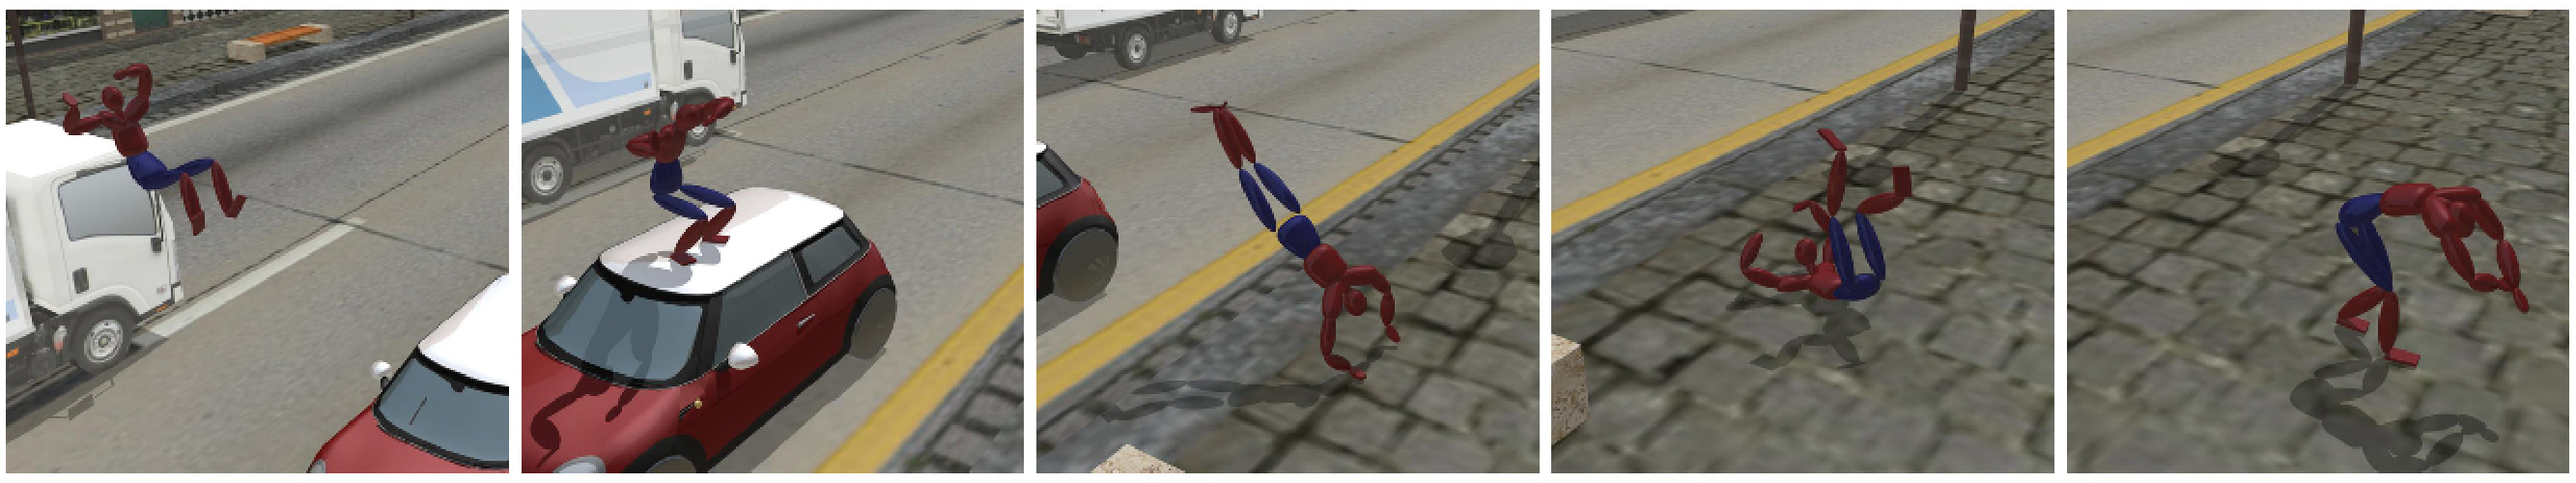
\includegraphics[width=\linewidth]{images/falling1_teaser}
  \caption{A simulated character lands on the roof of a car, 
    leaps forward, dive-rolls on the sidewalk, 
    and gets back on its feet, all in one continuous motion.}
 \label{fig:landingOverview}
\end{figure}


\section{Multi-contacts Falling Motion Control for a Humanoid Robot}

\subsection{Problem Description}

In this section, we propose to develop a safe falling controller for 
humanoid robots, which ensures the safety of the robots from the
large external perturbations.
Our approach is using the simulation samples for optimizing the controller
to handle complex changes of contacts from highly dynamic fallings.
By breaking a fall into a sequence of multiple contact, like ``UKEMI'' of Judo,
we expect the robot to endure larger external perturbations.
In addition, our simulation-based algorithm allows us to incorporate
an arbitrary objective function so that we can prioritize the body parts
to be protected.

The development of a safe falling controller requires design decisions
on when to detect the falling and how to evaluate the damages from falling.
In this proposal, we assume that the falling can be easily detected 
by observing acceleration of the center of mass and the 
falling controller will be activated after ?? seconds.
Evaluating the damages from the falling might be an interesting problem
to us, because it will dramatically affect the optimal control policy.
We plan to measure the damages on the bodies and joints
as contact forces and joint constraint forces, which might be
scaled to select more important ones to be protected.
Therefore, the objective function of our opitmization is accumulated body
damages and joint stresses while ignoring the negligible value
under the threshold.

\subsection{Related Work}

Safe falling and landing for bipeds is a topic that
receives broad attention in many disciplines. Robotic researchers are
interested in safe falling from standing height for the purpose of
reducing damages on robots due to accidental falls. Previous work has
applied machine learning techniques to predict falling
\cite{Kalyanakrishnan:2011:LPH}, as well as using an abstract model to
control a safe fall
\cite{Fujiwara:2002:FMC,Fujiwara:2007:OPF,Yun:2009:SFH}. 
In contrast to the related work in robotics, we use simulation samples
with detailed robot models to generate the optimal control policy.
The main advantage of using simulation is that it can capture
complex and arbitrary changes of contacts, which is hard to be 
formulated with an abstract model.
We draw inspiration from kinesiology literature and sport practitioners. 
In particular, the techniques developed in freerunning and parkour 
community are of paramount importance for designing landing control 
algorithms capable of handling arbitrary scenarios
\cite{Edwardes:2009:TPF,HLJ:2011:URL}. 

\subsection{Algorithm}

\paragraph{Optimization for a single scenario}

As the simplified version of the problem, we first develop the falling
controll for a single scenario, which starts from the given initial 
state.
For instance, the robot starts from its initial standing pose and 
being push its head backward for 0.1 second with 10N force.
When we know the parameterization of the controller, optimizing
control parameters for the given scenario can be easily solved
by various optimization techniques, such as 
Covariance Matrix Adaptation (CMA) \cite{Hansen:2004:CMA}).
After solving one instance of the scenarios, we can use the solution
as the guidance for the rest of the scenarios.

However, finding the proper parameterization of the controller
is a very difficult problem which usually requires a lot of prior knowledge.
In fact, there exist numerous control options in robotics, such as
pose control, torque control, virtual force control using Jacobian
Transpose, and so on.
Even one of the option, a pose control has an infinite number of choices for
representing its joint trajectories with splines.
Indeed, the selection of control dimension has a huge impact on the
result: we tested two parameterization of controller: a pose tracking 
with linear segments and bezier curves, which the latter has four times
more degrees of freedom than the former.
The optimization indicates that the bezier curve gives us 
much better results, which is one third of maximum impact
comparing to the linear control (Figure ??).

Therefore, our short term goal is finding the proper parameterization
of the controller.
One intuition from the previous falling and landing project is
momentum planning can be a simple and robust solution, so finding the 
proper momentum trajectory with an abstract model would be 
a promising approach.
Another potential approach is incrementally finding the control 
parameterization. 
In this approach, we search over the optimal parameterization by 
mutating the control dimension with genetic algorithm.
The value of each control dimension will be determined by solving
the optimization problem with the standard technique, like CMA.


\paragraph{Policy generation for multiple scenarios}

\subsection{Results}

\paragraph{Environment Setup}

\paragraph{Preliminary Results}



\chapter{Human-guided learning \protect\\ of dynamic motions}

\indent

In this section, we propose human-guided learning frameworks for
dynamic motor skills of virtual characters and real robots.
In the previous project, we introduced an intuitive and 
interactive system for developing dynamic controllers 
of virtual characters,
inspired by human learning process \cite{fitts:1967:hp}.
Further, under the paradigm of ``Learning from Demonstration''
in robotics,
we plan to extend/modify the training system to guide 
a motor skill acquition process of real robots, which
takes both task demonstrations and high-level instructions as inputs.

\section{Prior Work: Iterative Training Of Dynamic Skills Inspired By Human Coaching Techniques}

\indent

In our prior work \cite{Ha:2014:ITD},
we introduced an intuitive and interactive framework for developing 
dynamic controllers inspired by how humans learn dynamic motor
skills through progressive process of coaching and practices. 
The user only needs to provide a primitive initial controller and
high-level, human-readable instructions as if
she is coaching a human trainee, while the character has the ability
to interpret the abstract instructions, accumulate the knowledge from
the coach, and improve its skill iteratively. We introduce ``control
rigs'' as an intermediate layer of control module to facilitate the
mapping between high-level instructions and low-level control
variables. Control rigs also utilize the human coach's knowledge to
reduce the search space for control optimization. In addition, we
develop a new sampling-based optimization method, Covariance Matrix
Adaptation with Classification (CMA-C), to efficiently compute control
rig parameters. Based on the observation of human ability to ``learn
from failure'', CMA-C utilizes the failed simulation trials to
approximate an infeasible region in the space of control rig
parameters, resulting a faster convergence for the CMA
optimization. 
Without using motion trajectories, or tuning any parameters,
We demonstrate the design process of complex dynamic
controllers using our framework, including precision jumps, turnaround
jumps, monkey vaults, drop-and-rolls, and wall-backflips 
(\figref{training1_teaser}).


\begin{figure}[htbp]
\center
  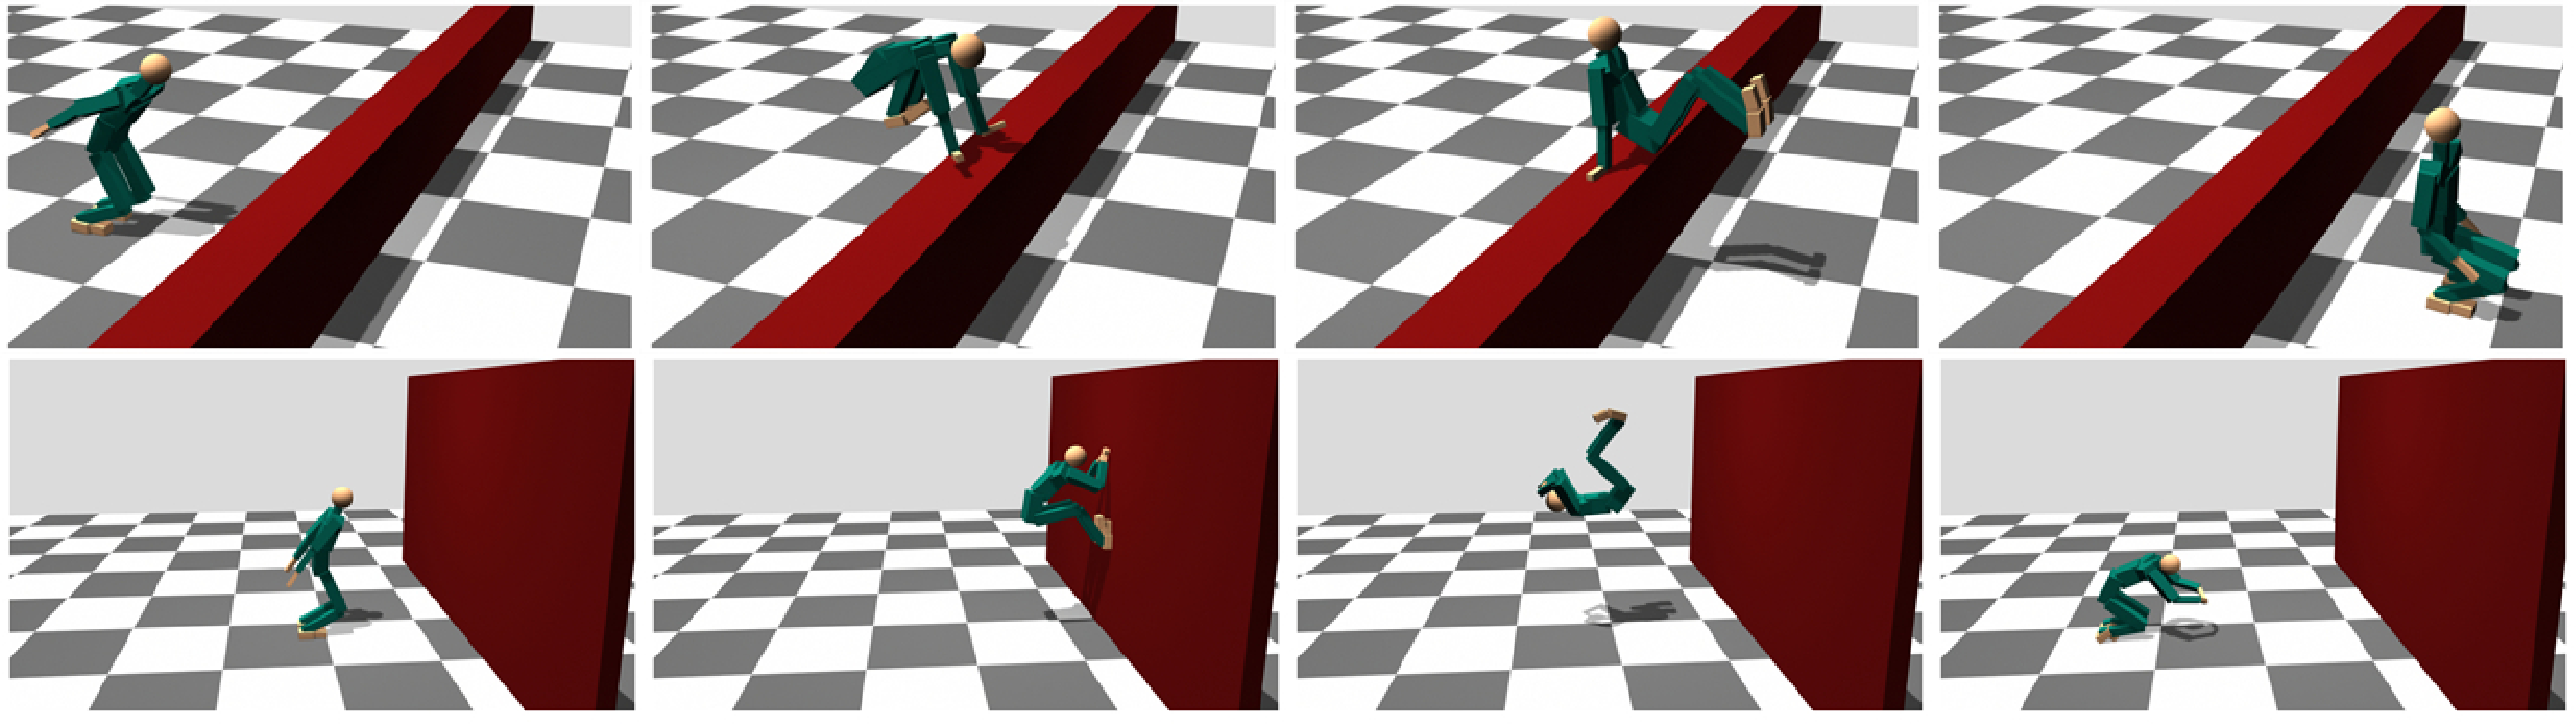
\includegraphics[width=\linewidth]{images/training1_teaser}
  \caption{The results from our previous work
    \cite{Ha:2014:ITD}:
    monkey vault (Top) and wall-backflip (Bottom).}
 \label{fig:training1_teaser}
\end{figure}


\section{Learning Dynamic Skills for a Humanoid Robot}

\subsection{Problem Description}

\indent

In this section, we propose to develop a framework for learning
dynamic motor skills of humanoid robots from user-provided demonstrations 
and instructions.
Our motivation is that both demonstrations and instructions are
common ways to guide a human-trainee, as we can see in a lot of
online tutorial videos.
In our framework, a coach demonstrates a set of example task motions
and records joint or mementum trajectories.
However, for full-body dynamic motor skills, recorded trajectories cannot 
be directly applied to the robot due to the different dynamics 
between a coach and the robot.
To interprete the demonstrated example motions properly,
we use high-level instructions which map the motions
to a proper control space, such a low-dimensional torque space 
or a control rig space \cite{Ha:2014:ITD} 
that suggested in our previous work.
Finally, we derive a robust control policy from the interpreted
demonstration set by learning the best action for the given state.
As a result, we can demonstrate a full-body dynamic motor skills
of humanoid robots under the guidance of human coach.

\subsection{Related Work}

\indent

Learning from demonstration (LfD), also known as programming by demonstration,
has been an attractive paradigm for training motor skills to robots.
In this paradigm, a set of examples are provided by human teachers,
and an optimal policy is generated from such examples.
Since the early work of Kuniyoshi \etal \cite{kuniyoshi:1989:TBS},
it has been proven to be effective for training motor skills in
numerous task domains, including object manipulation 
\cite{Atkeson:1997:RLD,Calinon:2007:LRG,Ueda:2010:MNH},
navigation \cite{Konidaris:2011:RLD}, 
full-body motion generation \cite{Kulic:2011:ILF}, and so on.
To increase the robustness, the learned motor skills are further 
generalized using various machine learning techniques,
such as Gausian Mixture Model \cite{Calinon:2007:LRG} or
Motion Primitives \cite{Pastor:2009:LGM}.
However, full-body dynamic motor skills of humanoids have
not been fully examined yet, except the only few works on the
locomotion \cite{Nakanishi:2004:LDA},
which is our target task domain in this proposal.

\subsection{Algorithms}

\paragraph{Domain of learning}

Choosing the right domain of learning is a critical problem 
in ``Learning from Demonstration'' paradigm.
In the literature, one of the most common domains is a set of kinematic
trajectories in joint angles or task spaces.
For instance, Akgun \etal \cite{Akgun:2011:KLD} presented a framework
for learning object manipulation tasks, such as scooping, pouring, or 
placement, from the kinematic keyframe data using 
Sequential Pose Distributions (SPD).
However, joint or torque trajectories cannot be directly applied to the
dynamic skills of the robots  due to the different dynamic properties 
of a coach and a trainee, which can make a huge impact on the motion
with just minor deviations.

To overcome this issue, we hypothesize that learning in the control domain,
instead of the kinematic domain, would allow more straight-forward 
learning and roboust behaviors.
Here is an illustrative example:
joint trajectories of rolling motions for human and a
robot might be very different from each other due to the different
dimensions, but semantically both motions consist of 
three sub-stages: leaning, kicking, and stopping.
To this end, we combine the demonstration with user provided high-level
instructions, which can help us to identify the proper domain of controls.
The control domain can be a projected low-dimensional control space using
Principal Component Analysis (PCA) or a control rig space, as defined
in the previous work \cite{Ha:2014:ITD}.
Especially, control rigs can project the high-dimensional control into
lower dimensions by control multiple degrees of freedoms simultaneously,
and can be easily constructed from a sequence of human-readble 
instructions.
For instance, ``MOVE DOWN'' instruction will add a ``Leg-distance'' rig,
which controls the distance between the root and feet using an inverse
kinematics solver.
We hope that high-level instructions combined with demonstrations
can expedite the learning from user demonstrations 
for dynamic motor skills.

\paragraph{Optimization}

To apply to the trainee, a robot, the control parameters are required to be
optimized to the new dynamic character to follow the user-provided 
examples and instructions.
For the simplest case, 
the optimization of the parameters in the simulation environtment
might be easily solved with a standard sampling-based optimization
techniques, such as CMA.
However, deploying the controller to the real robot with hardwares
may require the additional robustness of the controller
due to the noise on the sensors and servos.
Therefore, we may need to ensure the robustness of the solution,
which can be potentially done by testing the objective value 
with minor perturbations as suggested in Ha \etal \cite{Ha:2013:PSB}.

\subsection{Expected Results}

\begin{figure}[htbp]
\center
  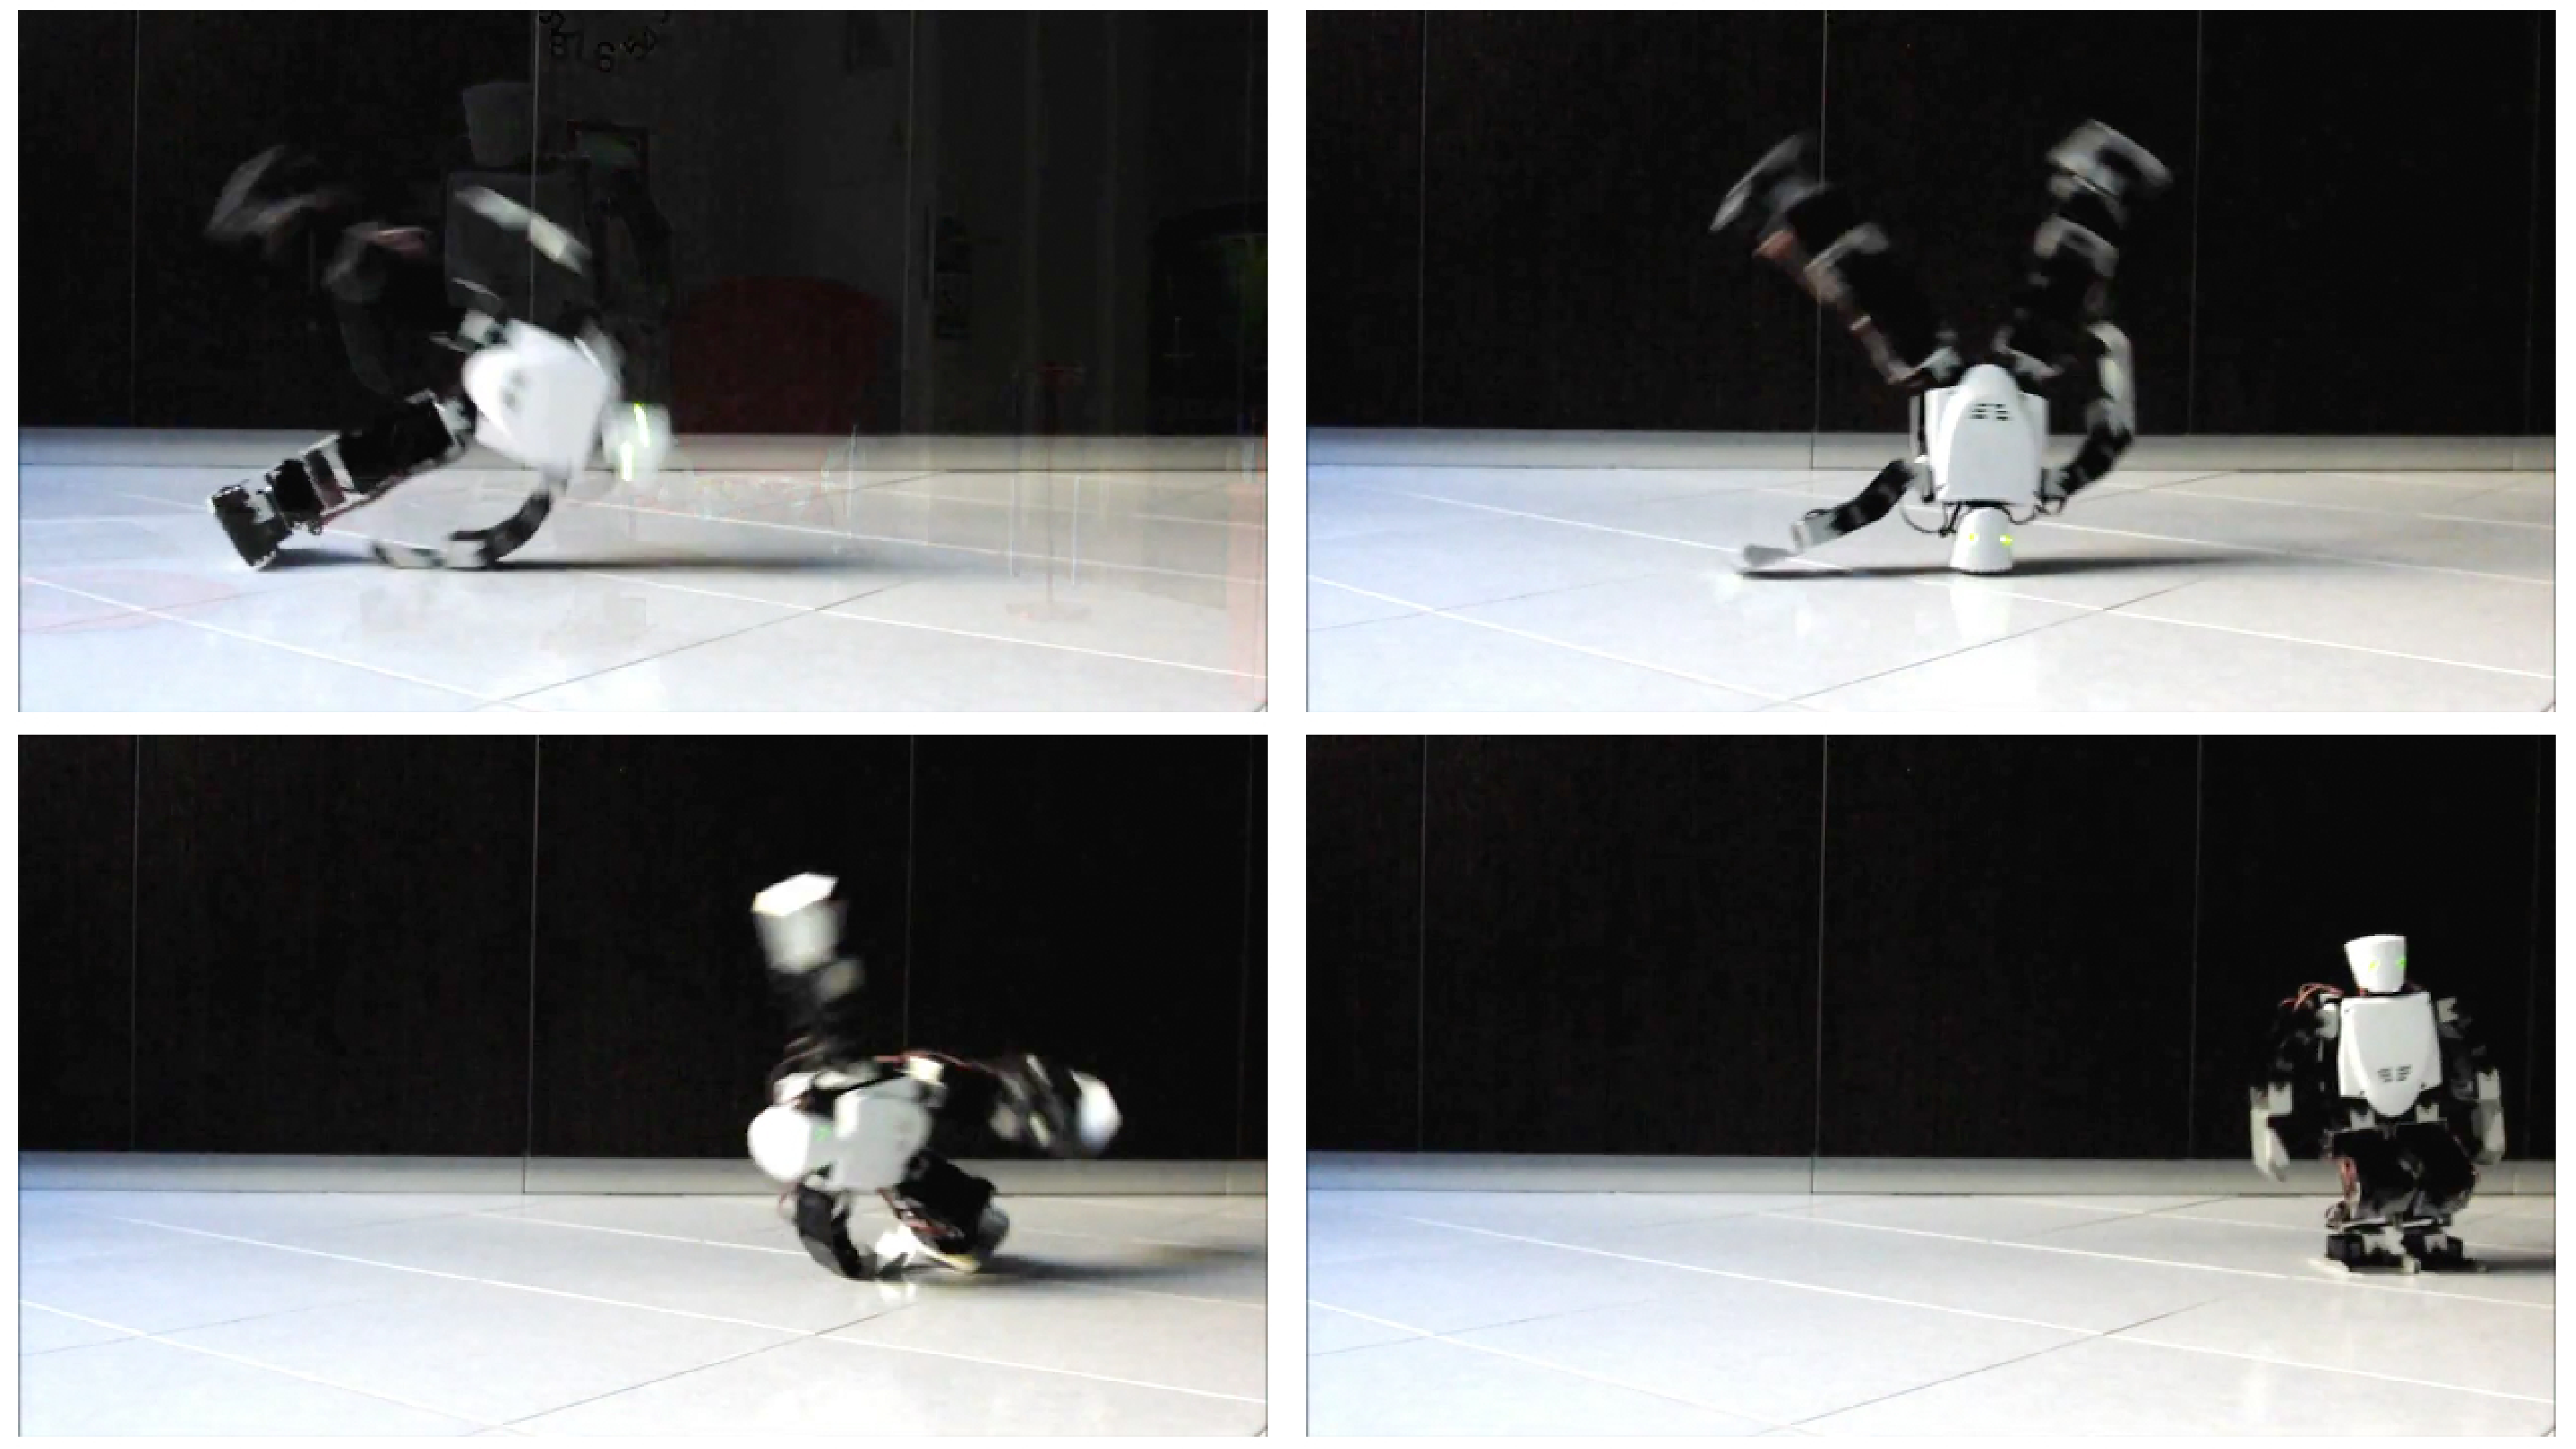
\includegraphics[width=5.0in]{images/training2_cartwheel}
  \caption{Manually scriptted cartwheel of Robovie \cite{Youtube-Robovie-X}.}
 \label{fig:cartwheel}
\end{figure}

\indent

The goal of this project is learning dynamic motor skills
from the user-provided demonstrations and instructions.
Again, we select a table-top humanoid robot, 
Robovie-X Standard (17 DoFs), as a subject.
We consider various target motions 
such as rolling, cartwheel, or yoga-balancing,
currently which manually developed by providing a sequence of keyframes 
(\figref{cartwheel}).

The demonstration of dynamic motor skills would be followed by
additional analyses.
For instance, joint or torque trajectories of trained motions 
can be analyzed to compare the motions of the coach and the robot.
Further, the trajectories of trained motions in kinematic domain 
and control domain can be analyzed to compare our framework
with previously suggested frameworks.


\chapter{Timeline for proposed research}

\begin{itemize}
  \item 2014, Apr: present proposal to committee
  \item 2014, Apr - May: work on the optimal control of the falling project
  \item 2014, May - Sep: work on the policy generation of the falling project
  \item 2014, Sep: submit the falling project to ICRA 2015
  \item 2014, Sep - 2015, Jul: work on the learning project
  \item 2015, May - Aug: write thesis
  \item 2015, Aug: defense thesis
  \item 2015, Sep: submit the learning project to ICRA 2016
\end{itemize}


%% \section{Concepts}
%% This is where we talk about the concepts behind the dissertation.
%% \subsection{Primary Concept}
%% This is the primary concept.
%% \subsection{Secondary Concept}
%% This is the secondary concept.
%% \subsubsection{Even more secondary}
%% This is really not all that important.

%% \begin{table}
%% \caption{A table, centered.}
%% \begin{center}
%% \begin{tabular}{|l|r|}
%%   \hline 
%% Title & Author \\
%% \hline
%% War And Peace & Leo Tolstoy \\
%% The Great Gatsby & F. Scott Fitzgerald \\ \hline
%% \end{tabular}
%% \end{center}
%% \end{table}


%%
%% \chapter{Previous Work}
%% Some other research was once performed.

%% \begin{figure}
%% \caption{A first figure.}
%% \end{figure}

%% \begin{figure}
%% \caption{A second figure.}
%% \end{figure}
%%
%% \chapter{Conclusion}

%% \nocite{*}
%% We need this since this file doesn't ACTUALLY \cite anything...
%%
\appendix
%% \chapter{Some Ancillary Stuff}

%% Ancillary material should be put in appendices, which 
%% appear just before the bibliography. 

\begin{postliminary}
\references

%% \postfacesection{Index}{%
%% %%             ... generate an index here
%% %%         look into gatech-thesis-index.sty
%% }
%% \begin{vita}
%% Perry H. Disdainful was born in an insignificant town
%% whose only claim to fame is that it produced such a fine
%% specimen of a researcher.
%% \end{vita}

%% \begin{abstract}
%%   Haha, my thesis proposal is awesome. Please accept this!
%%   This is the abstract that must be turned in as hard copy to the
%%   thesis office to meet the UMI requirements. It should \emph{not} be
%%   included when submitting your ETD. Comment out the abstract
%%   environment before submitting. It is recommended that you simply
%%   copy and paste the text you put in the summary environment into this
%%   environment. The title, your name, the page count, and your
%%   advisor's name will all be generated automatically.
%% \end{abstract}


\end{postliminary}


\end{document}
